\section{Simulation}

\frame
{
\frametitle{Simulation}
\begin{itemize}
	\item GA
	\begin{itemize}
		\item Generation = 50
		\item Population size = 200
		\item Crossover Probability = 0.6
		\item Mutation Probability = 0.0.1
	\end{itemize}
	\item CSA
	\begin{itemize}
		\item Generation = 50
		\item Population size = 200
		\item Percentage of new population = 0.6
		\item Hyper-mutation = 0.0.1
	\end{itemize}
\end{itemize}
}

\frame
{
\frametitle{Simulation}
\framesubtitle{A. Simulation Results of Complex Environment}
\begin{center}
	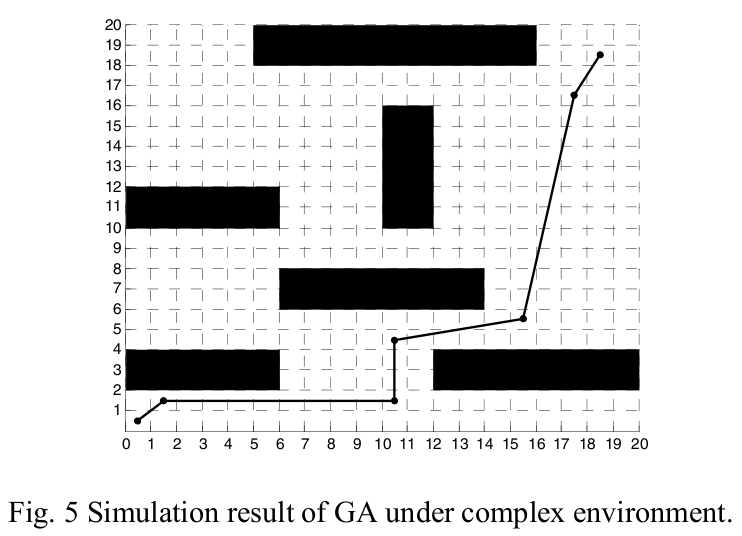
\includegraphics[width=0.8\textwidth]{img/garesult}
\end{center}
}

\frame
{
\frametitle{Simulation}
\framesubtitle{A. Simulation Results of Complex Environment}
\begin{center}
	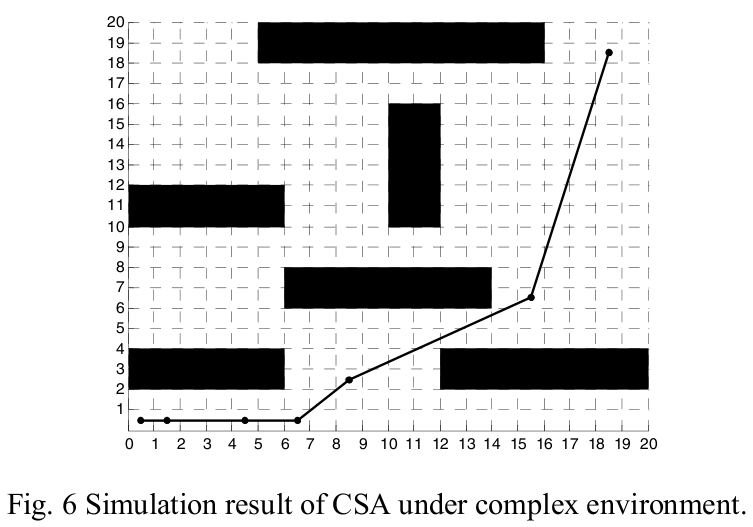
\includegraphics[width=0.8\textwidth]{img/csaresult}
\end{center}
}
\frame
{
\frametitle{Simulation}
\framesubtitle{A. Simulation Results of Complex Environment}
\begin{center}
	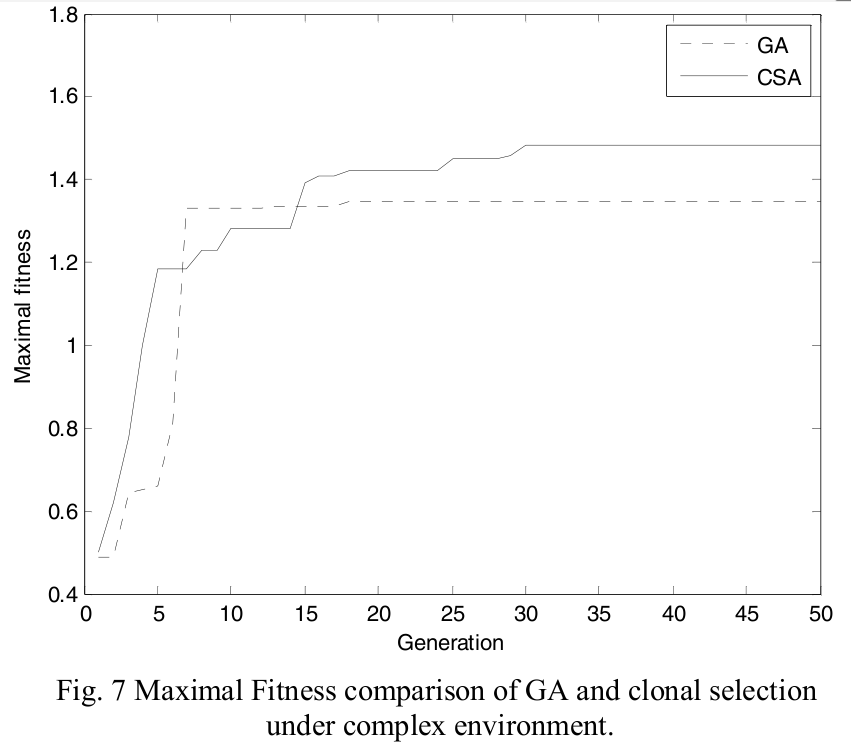
\includegraphics[width=0.7\textwidth]{img/maximal}
\end{center}
}
\frame
{
\frametitle{Simulation}
\framesubtitle{A. Simulation Results of Complex Environment}
\begin{center}
	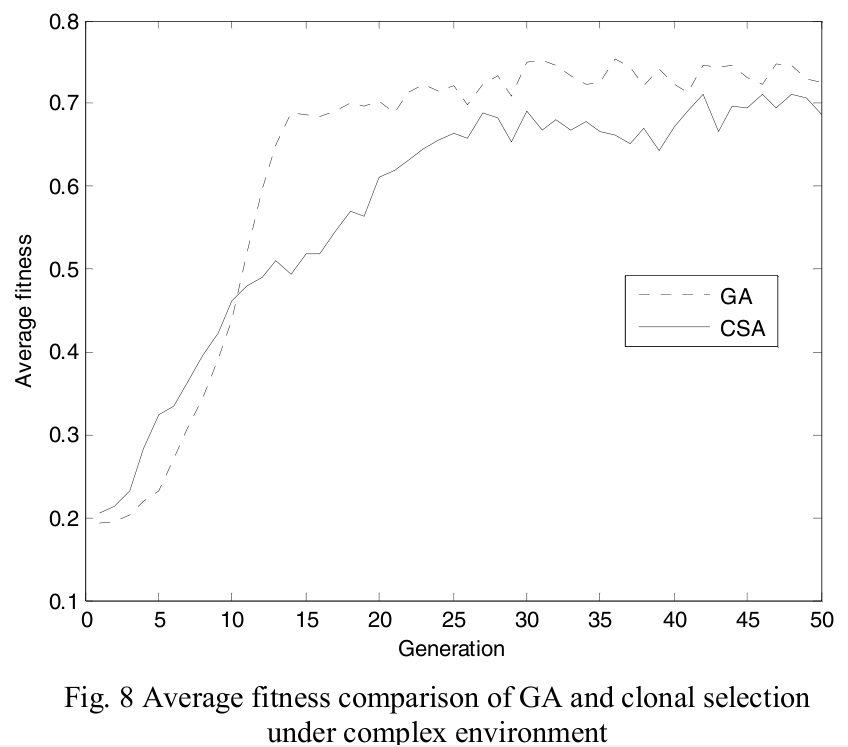
\includegraphics[width=0.7\textwidth]{img/average}
\end{center}
}

\frame
{
\frametitle{Simulation}
\framesubtitle{B. Simulation Results of U Type Environment}
\begin{center}
	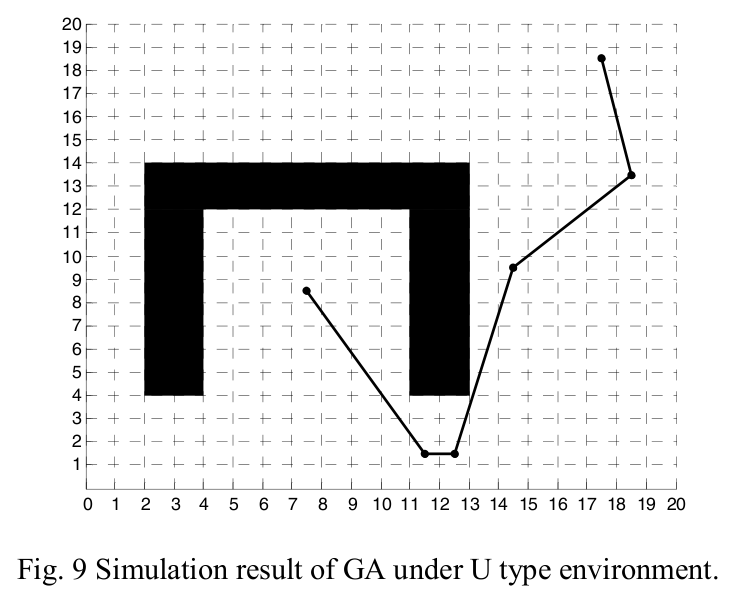
\includegraphics[width=0.7\textwidth]{img/garesult2}
\end{center}
}

\frame
{
\frametitle{Simulation}
\framesubtitle{B. Simulation Results of U Type Environment}
\begin{center}
	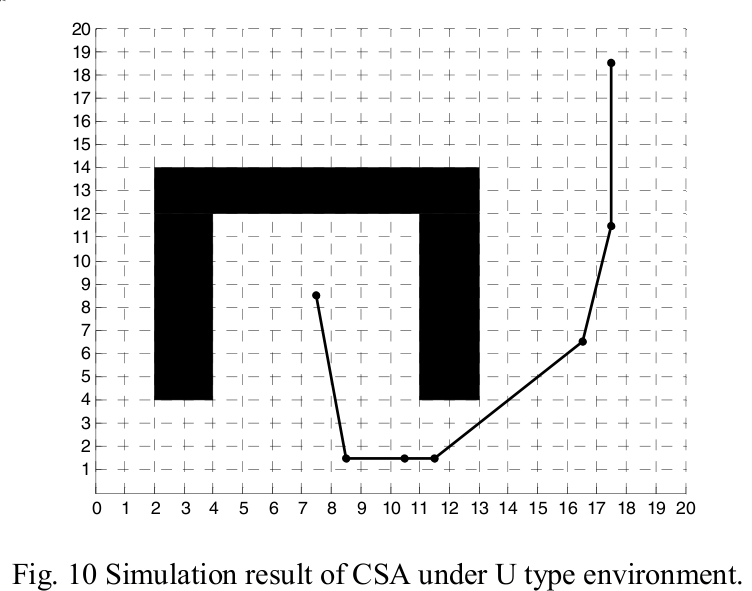
\includegraphics[width=0.7\textwidth]{img/csaresult2}
\end{center}
}
\frame
{
\frametitle{Simulation}
\framesubtitle{B. Simulation Results of U Type Environment}
\begin{center}
	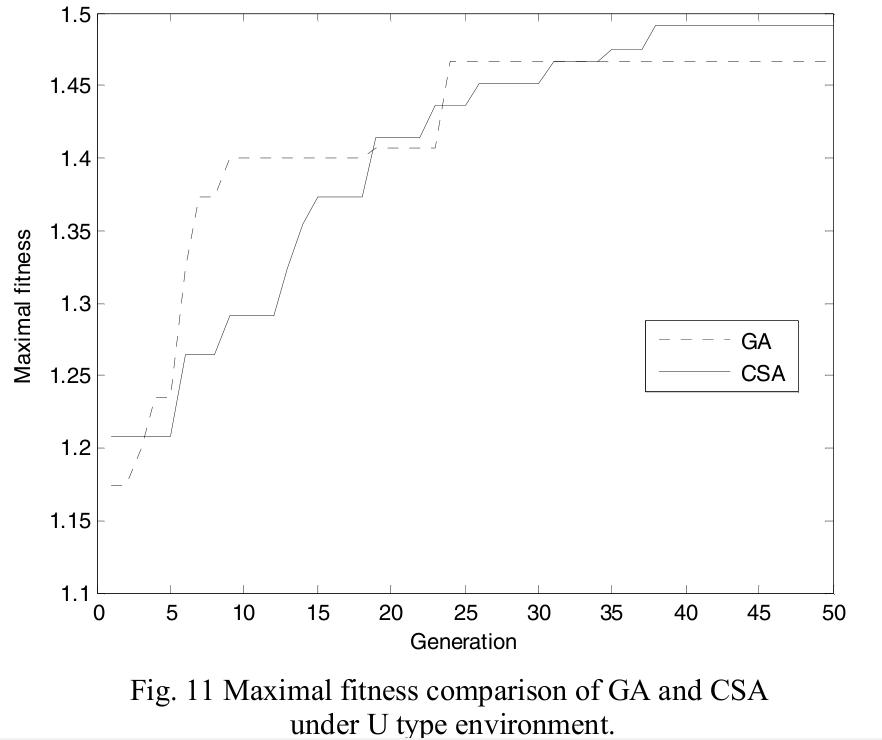
\includegraphics[width=0.7\textwidth]{img/maximal2}
\end{center}
}
\frame
{
\frametitle{Simulation}
\framesubtitle{B. Simulation Results of U Type Environment}
\begin{center}
	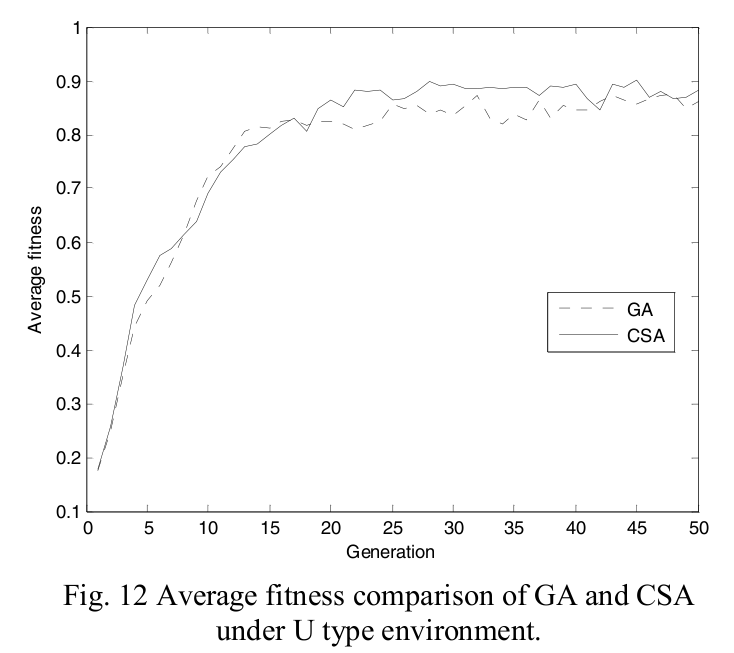
\includegraphics[width=0.7\textwidth]{img/average2}
\end{center}
}
